\setcounter{figure}{0}

\section{27th August 2023: Love, sex and marriage}
\subsection*{Text: Song of Solomon 3:6-5:1}
  \begin{quote}
    [6] What is that coming up from the wilderness
        like columns of smoke,
    perfumed with myrrh and frankincense,
        with all the fragrant powders of a merchant?
    [7] Behold, it is the litter of Solomon!
    Around it are sixty mighty men,
        some of the mighty men of Israel,
    [8] all of them wearing swords
        and expert in war,
    each with his sword at his thigh,
        against terror by night.
    [9] King Solomon made himself a carriage
        from the wood of Lebanon.
    [10] He made its posts of silver,
        its back of gold, its seat of purple;
    its interior was inlaid with love
        by the daughters of Jerusalem.
    [11] Go out, O daughters of Zion,
        and look upon King Solomon,
    with the crown with which his mother crowned him
        on the day of his wedding,
        on the day of the gladness of his heart.


        He

    [1] Behold, you are beautiful, my love,
        behold, you are beautiful!
    Your eyes are doves
        behind your veil.
    Your hair is like a flock of goats
        leaping down the slopes of Gilead.
    [2] Your teeth are like a flock of shorn ewes
        that have come up from the washing,
    all of which bear twins,
        and not one among them has lost its young.
    [3] Your lips are like a scarlet thread,
        and your mouth is lovely.
    Your cheeks are like halves of a pomegranate
        behind your veil.
    [4] Your neck is like the tower of David,
        built in rows of stone;
    on it hang a thousand shields,
        all of them shields of warriors.
    [5] Your two breasts are like two fawns,
        twins of a gazelle,
        that graze among the lilies.
    [6] Until the day breathes
        and the shadows flee,
    I will go away to the mountain of myrrh
        and the hill of frankincense.
    [7] You are altogether beautiful, my love;
        there is no flaw in you.
    [8] Come with me from Lebanon, my bride;
        come with me from Lebanon.
    Depart from the peak of Amana,
        from the peak of Senir and Hermon,
    from the dens of lions,
        from the mountains of leopards.


    [9] You have captivated my heart, my sister, my bride;
        you have captivated my heart with one glance of your eyes,
        with one jewel of your necklace.
    [10] How beautiful is your love, my sister, my bride!
        How much better is your love than wine,
        and the fragrance of your oils than any spice!
    [11] Your lips drip nectar, my bride;
        honey and milk are under your tongue;
        the fragrance of your garments is like the fragrance of Lebanon.
    [12] A garden locked is my sister, my bride,
        a spring locked, a fountain sealed.
    [13] Your shoots are an orchard of pomegranates
        with all choicest fruits,
        henna with nard,
    [14] nard and saffron, calamus and cinnamon,
        with all trees of frankincense,
    myrrh and aloes,
        with all choice spices—
    [15] a garden fountain, a well of living water,
        and flowing streams from Lebanon.


    [16] Awake, O north wind,
        and come, O south wind!
    Blow upon my garden,
        let its spices flow.


    She

    Let my beloved come to his garden,
        and eat its choicest fruits.


    He

    [1] I came to my garden, my sister, my bride,
        I gathered my myrrh with my spice,
        I ate my honeycomb with my honey,
        I drank my wine with my milk.


    Others

    Eat, friends, drink,
        and be drunk with love!
  \end{quote}
\subsection*{Notes}
\begin{itemize}
  \item{In the song “fly me to the moon”, there is a lot of imagery but the main point is just the person saying that he/she wants to he loved. All the “fly me to the moon and let me sit among the stars” stuff. Similarly, there is a lot of imagery here but here we need to find the message behind the imagery.}
  \item{The text starts with Solomon’s wedding carriage. Probably Solomon here is just used to depict an ideal “prince charming”, and all of the description here about Solomon is saying like the groom is regal, fierce (lol), and a protector, just like Solomon. }
  \item{The text then talks about the bride. The text first starts with a description of the bride’s eyes, and then moves down to describe her hair, her teeth, her neck, and then down to her breasts. After describing her breasts, he then talks about going to the mountain and etc with her lol. Probably this is the groom expressing a desire for privacy and physical intimacy with his bride.}
  \item{Then v12-16 is the actual physical intimacy lol. The garden here in ancient near eastern culture refers to a woman’s genitals. Note: at first the woman’s garden is referred to as locked (so the woman is a virgin), then thereafter the woman asks the man to enter her garden (wow), i.e sexual union, and the man gladly does so. Ancient near eastern culture focuses on the woman’s virginity (patriarchal culture), and we can see this in God’s Law too in the OT. But we no longer live in these days (i.e, prizing the woman's virginity more importantly than the man's!).}
  \item{Song of solomon is about the love between man and woman, and this love is epitomised in the sexual union between man and woman. }
  \item{Sex is something God created to be enjoyed by a man and a woman in marriage, we see that in Eden. But because of sin, the intimacy that a man and a woman is lost (they were ashamed), and now sex is corrupted by sin. That sex is corrupted can be seen by how in ancient near eastern culture, there were things like temple prostitutes etc. People still knew that sex is of divine origin, but they think that sex with the idols (as mediated by the prostitutes) is a thing. Then today, there are two extremes; one extreme says sex is dirty and bad and only to be used as a vehicle for baby-making. The other extreme says sex is to be openly and freely enjoyed with all people and that babies are a hindrance.}
  \item{In our text, we see a man and woman in a garden (v12-16), and they had joy in their marital union, which is in a sense, a redeeming of what was lost in Eden.}
  \item{Marriage as an institution has inherent honour and dignity, which is why in many cultures, they have something similar to Solomon’s entourage as described here. E.g, in Chinese culture, we have the many cars during the gatecrash lol. Or more generally, weddings are quite extravagant. That is not wrong even for us christians, but that must be done in the right spirit. An extravagant wedding cannot be done as a flaunt of wealth or what, that is wrong. The right spirit is that the wedding must be done as a show of love between the couple and also as gratitude to the parents (e.g SoS 3:11). If we have the means to and if our heart is right (as per mentioned above), then a more expensive wedding is ok. }
  % \item{\begin{figure}[H]
  %   \centering
  %   % 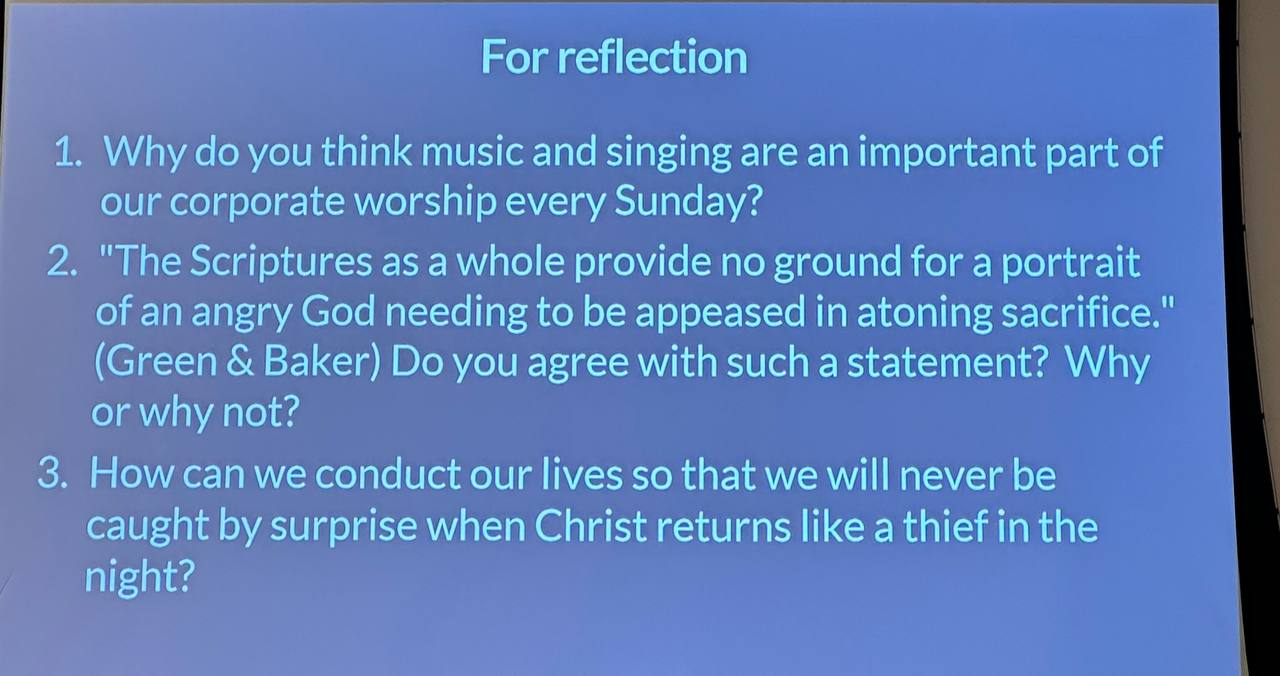
\includegraphics[width=0.8\textwidth, trim={0cm 0cm 0cm 0cm},clip]{Figures/marchSermon4Reflections.jpg}
  %   \includegraphics[width=0.8\textwidth, trim={0cm 0cm 0cm 0cm},clip]{example-image-a}
  %   \caption[]{Reflection questions for this sermon}
  %   \label{}
  % \end{figure}}
\end{itemize}